\pagehead{Recommendations}

If you're looking to dive into the library's collection but are having
trouble deciding where to start, here are some recommendations from
the committee:

\bookrec{Hetty Symes}{The Mistborn Saga}{Brandon Sanderson}{What a fantastic magic system, I feel like I can actually understand it. Great character development and world-building. If you want to try out Brandon Sanderson's works, this is a great starting place for you.}

\bookrec{Clifford Chan}{Children of Time}{Adrian Tchaikovsky}{Theory of evolution but with spiders. Won the Arthur C. Clarke Award in 2016. Best sci-fi book I've read in ages.}

\bookrec{Hetty Symes}{Piranesi}{Susanna Clarke}{I started this because it was trending on Audible at the time. Absolutely loved it. The highlight for me was the ethereal descriptions of the labyrinth the MC lives in. Don't expect a fast-paced plot line but rather an ongoing, scenic adventure with hints of mystery.}

\bookrec{Juairiyah Raqib}{Discworld}{Terry Pratchett}{Only 41 novels – if you read 1 book a month you {\normalfont might} finish the series before you leave university.}

\bookrec{Hetty Symes}{The Lord of the Rings}{J. R. R. Tolkien}{You know what this is. It's long, but if you like beautiful passages describing nature and meticulous world-building then this is the trilogy for you. I read this after watching the films, and safe to say it did not disappoint.}

\bookrec{Clifford Chan}{Yumi and the Nightmare Painter}{Brandon Sanderson}{A fantastical, body-swapping romance inspired by Your Name, set in the Cosmere. One of the most emotionally impactful Sanderson books so far.}

\bookrec{Sam Shanker}{Worm}{John C. McCrae (Wildbow)}{A superhero web serial about cataclysmic events and a girl who controls bugs.}

\bookrec{Hetty Symes}{Circe}{Madeline Miller}{Finished this one last week. If you like learning about Greek mythology (which was me as a Percy Jackson fan) then I would recommend. Experience mythological events from a minor goddess' POV!}

\bookrec{Hetty Symes}{The Wandering Earth}{Cixin Liu}{Will this be my one Sci-Fi rec? I read it amongst a collection of other Liu Cixin short stories. He's most well-known for his series The Three-Body Problem (which I still plan on reading, though I did watch its C-drama that released this year - would recommend).}

\bookrec{Clifford Chan}{Project Hail Mary}{Andy Weir}{From the author of The Martian, a delightful hard sci-fi with some very fun ideas. The one book I'm certain both beginners and veterans of the genre will enjoy.}

\bookrec{Hetty Symes}{The Priory of the Orange Tree}{Samantha Shannon}{Is this the time to boast that I met the author at Comic Con in my first year? (and I was reading this book at the time!) Such a great fantasy book. There's a lot of world-building so prepare to be confused in the beginning. Has everything from pirates to dragons.}

\bookrec{Clifford Chan}{Gideon the Ninth}{Tamsyn Muir}{Lesbian necromancers in space solve a murder mystery. If that sounds like your thing, you're in for a treat!}\\

\begin{center}
    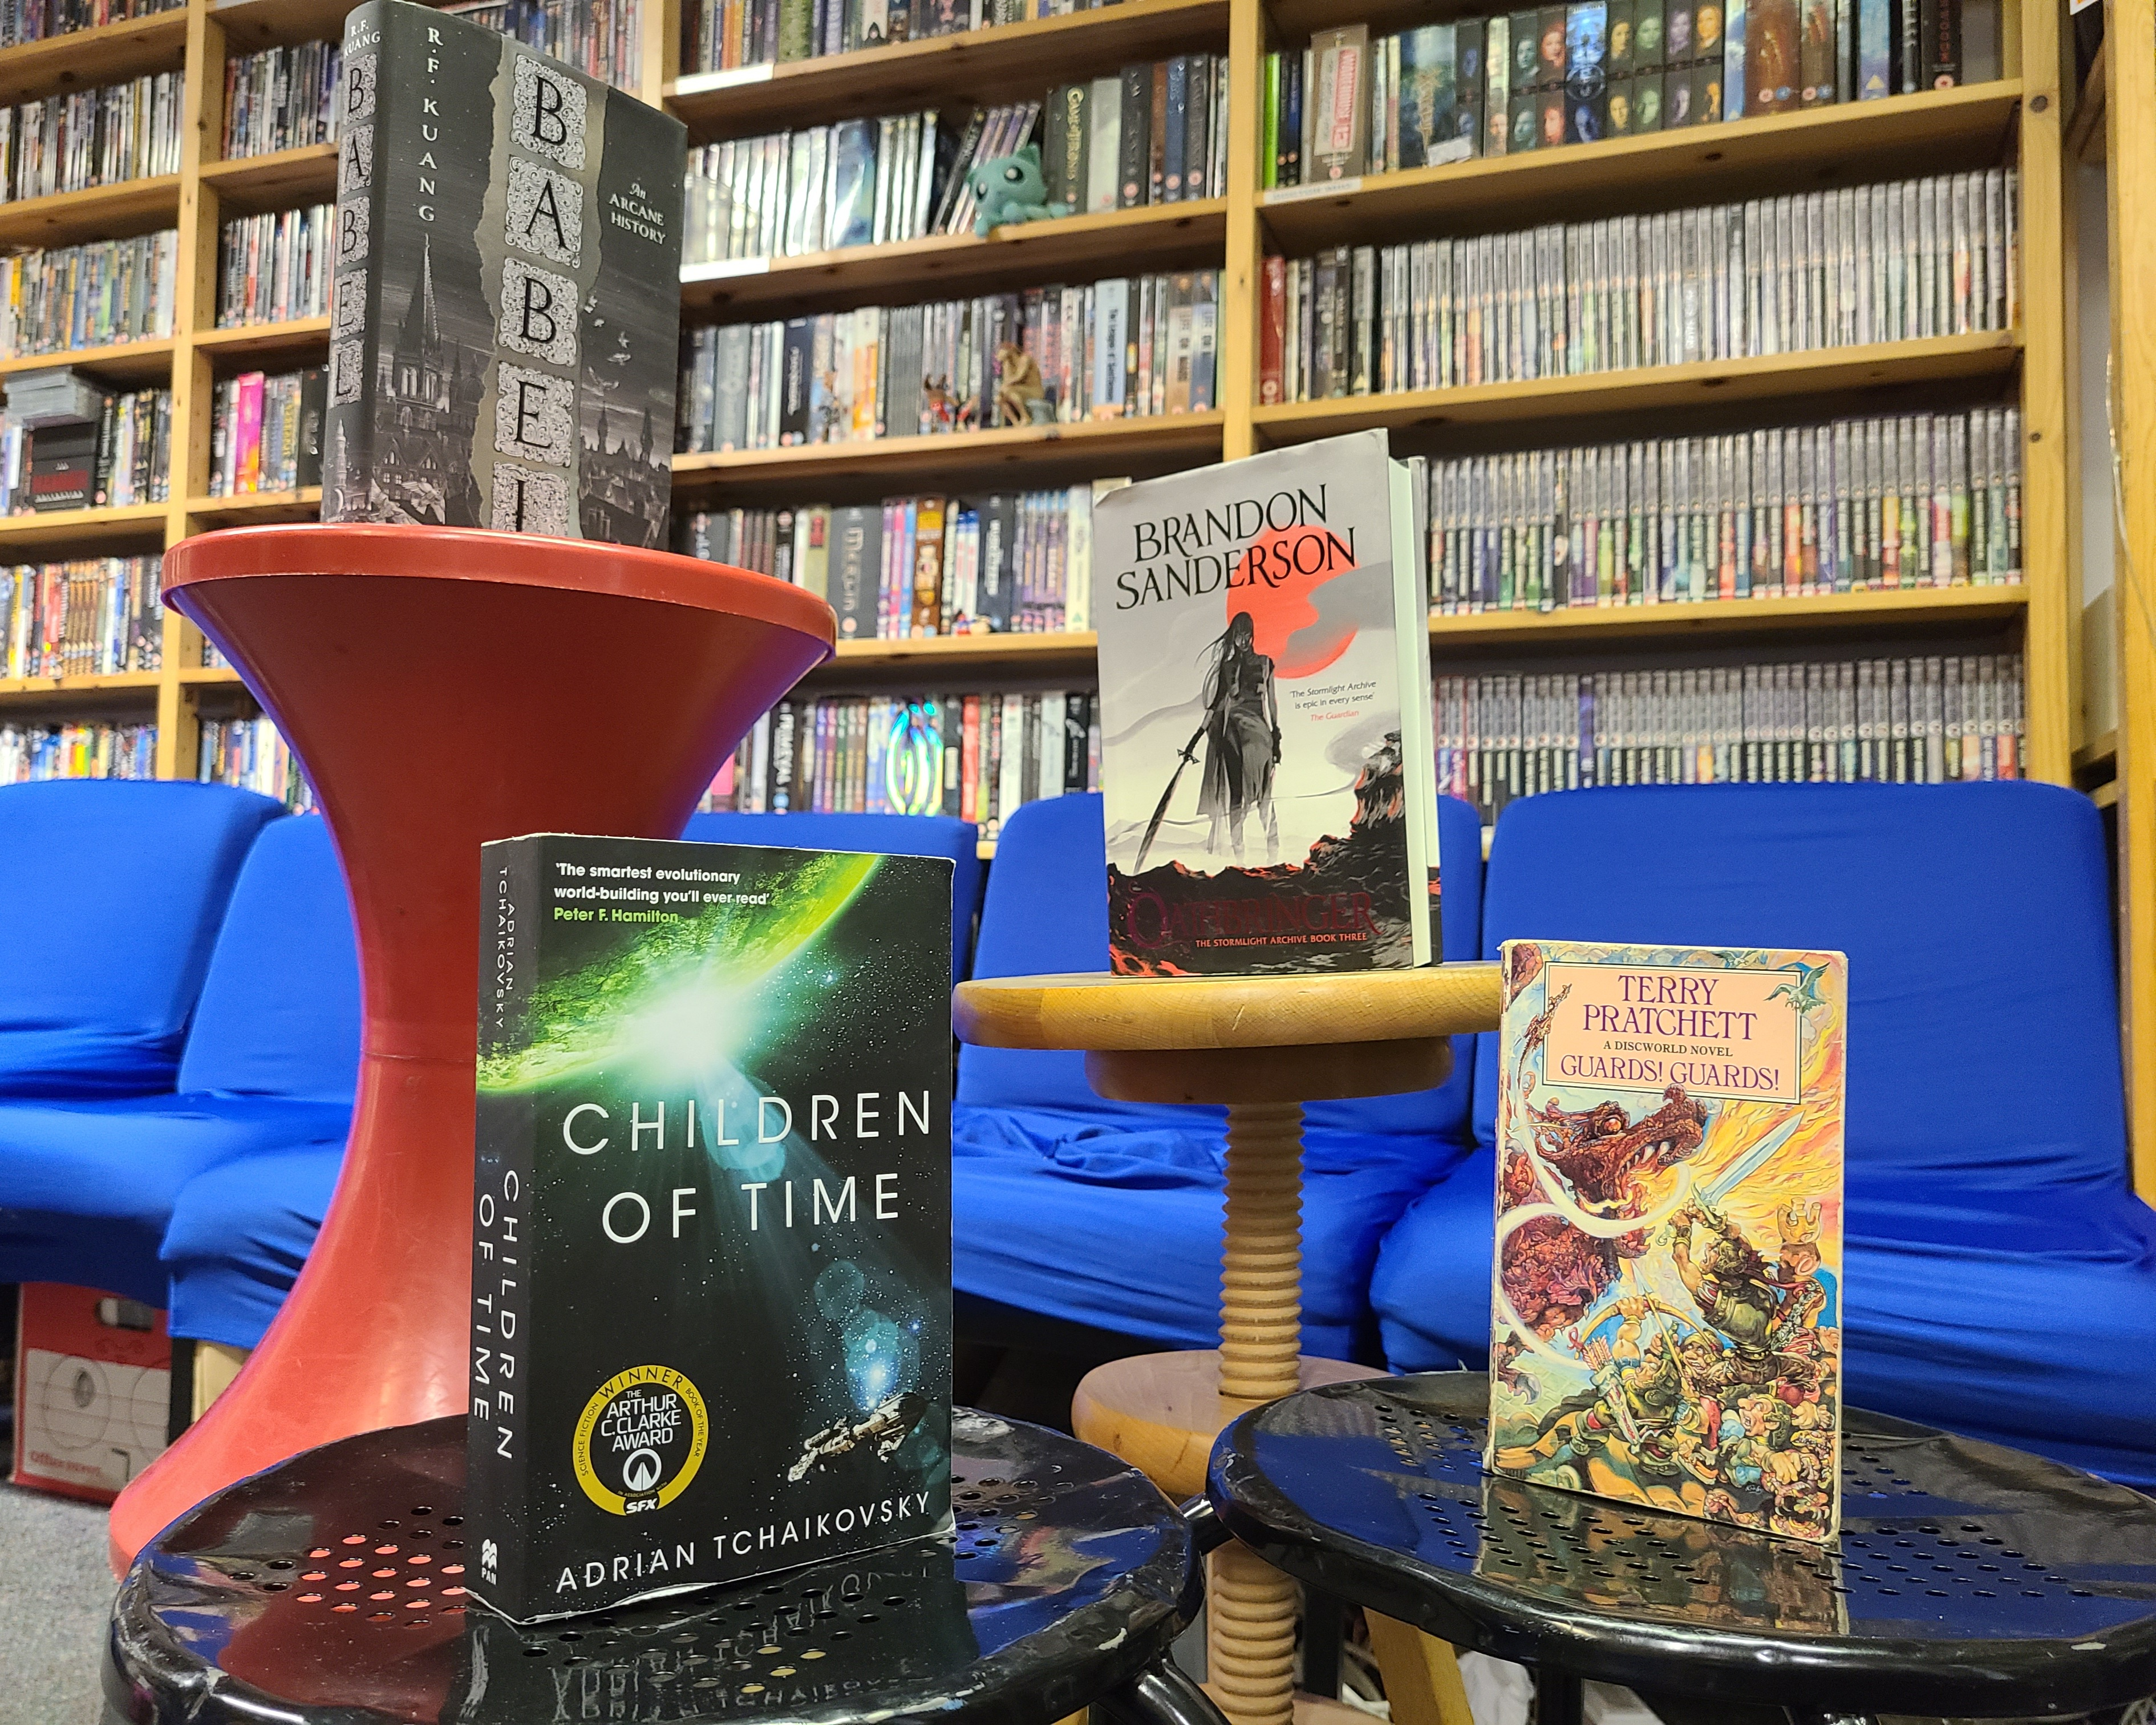
\includegraphics[width = 0.7\textwidth]{img/info/book-rec.png}
\end{center}